% ============================================================
%  RCC Agent-Based Model — Beamer Slideshow
% ============================================================
\documentclass[aspectratio=169,10pt]{beamer}

% ---- Theme & colours ----
\usetheme{Madrid}
\definecolor{tealblue}{RGB}{0,128,148}
\definecolor{darkteal}{RGB}{0,90,110}
\definecolor{lightteal}{RGB}{200,235,240}
\setbeamercolor{palette primary}{bg=tealblue,fg=white}
\setbeamercolor{palette secondary}{bg=darkteal,fg=white}
\setbeamercolor{palette tertiary}{bg=darkteal,fg=white}
\setbeamercolor{structure}{fg=tealblue}
\setbeamercolor{title}{fg=white,bg=tealblue}
\setbeamercolor{frametitle}{fg=white,bg=tealblue}
\setbeamercolor{block title}{bg=tealblue,fg=white}
\setbeamercolor{block body}{bg=lightteal,fg=black}

% ---- Clean presentation ----
\setbeamertemplate{navigation symbols}{}  % Remove nav clutter
\setbeamertemplate{footline}[frame number] % Clean page numbers

% ---- Packages ----
\usepackage[utf8]{inputenc}
\usepackage[T1]{fontenc}
\usepackage{booktabs}
\usepackage{amsmath,amssymb}
\usepackage{tikz}
\usetikzlibrary{arrows.meta,positioning,shapes.geometric,calc,fit}
\usepackage{graphicx}
\usepackage{array}
\usepackage{multirow}
\usepackage{hyperref}

% ---- Metadata ----
\title[RCC ABM]{Agent-Based Modeling of Renal Cell Carcinoma\\with Glucose Sensing}
\subtitle{A Repast4Py Implementation}
\author{Samuele Stronati}
\date{\today}
\institute{}

% ---- Outline at section start ----
\AtBeginSection[]{%
  \begin{frame}{Outline}
    \tableofcontents[currentsection]
  \end{frame}
}

% ============================================================
\begin{document}

% ---- Slide 1: Title ----
\begin{frame}[plain]
  \titlepage
\end{frame}

% ---- Slide 2: Outline ----
\begin{frame}{Outline}
  \tableofcontents
\end{frame}

% ============================================================
\section{Introduction \& Motivation}
% ============================================================

% ---- Slide 3: RCC Problem ----
\begin{frame}{Renal Cell Carcinoma --- The Clinical Challenge}
  \begin{columns}[T]
    \column{0.55\textwidth}
    \begin{itemize}
      \item 3\textsuperscript{rd} most common urological cancer
      \item $\sim$400\,000 new cases per year worldwide
      \item Metastatic 5-year survival $<15\%$
      \item Clear-cell RCC (ccRCC) accounts for $\sim$75\% of cases
      \item Strong sex differences:
        \begin{itemize}
          \item Incidence ratio $\approx 2{:}1$ (male : female)
          \item Females show better immunotherapy response
        \end{itemize}
    \end{itemize}

    \column{0.42\textwidth}
    \begin{block}{Key Facts}
      \small
      \begin{tabular}{@{}ll@{}}
        \toprule
        Metric & Value \\
        \midrule
        Incidence & 400k/yr \\
        M:F ratio & 2:1 \\
        5-yr survival & $<$15\% \\
        Main subtype & ccRCC \\
        \bottomrule
      \end{tabular}
    \end{block}
  \end{columns}
\end{frame}

% ---- Slide 4: Why ABM ----
\begin{frame}{Why Agent-Based Modeling?}
  \begin{columns}[T]
    \column{0.48\textwidth}
    \begin{block}{Strengths of ABMs}
      \begin{itemize}
        \item Natural representation of \textbf{heterogeneous} cell populations
        \item Capture \textbf{spatial dynamics} and local interactions
        \item \textbf{Emergent behaviour} arises from simple rules
        \item \textbf{In silico} experimentation --- fast, ethical, cheap
        \item Stochasticity matches biological variability
      \end{itemize}
    \end{block}

    \column{0.48\textwidth}
    \begin{block}{Limitations of ODE/PDE Models}
      \begin{itemize}
        \item Assume well-mixed populations
        \item Difficult to capture cell-level heterogeneity
        \item No spatial resolution
        \item Hard to model discrete events (mutation, death)
      \end{itemize}
    \end{block}
  \end{columns}
\end{frame}

% ---- Slide 5: Project Objectives ----
\begin{frame}{Project Objectives}
  \begin{enumerate}
    \item \textbf{Port Mesa $\rightarrow$ Repast4Py}: migrate the existing RCC ABM to a scalable MPI-based framework
    \item \textbf{Add glucose microenvironment}: 3D reaction--diffusion field modelling the Warburg effect
    \item \textbf{Validate against clinical data}: fit model to ARON-1 clinical survival outcomes
    \item \textbf{Bayesian optimisation}: tune 114 parameters with Optuna (TPE sampler, 250 trials)
    \item \textbf{Sex-specific analysis}: compare male vs.\ female immune dynamics under treatment
  \end{enumerate}
\end{frame}

% ============================================================
\section{Theoretical Core}
% ============================================================

% ---- Slide 6: ABM Formalism ----
\begin{frame}{ABM Formalism \& Repast4Py}
  \begin{columns}[T]
    \column{0.48\textwidth}
    \begin{block}{ABM Components}
      \begin{description}
        \item[Agents] autonomous entities with state \& rules
        \item[Environment] 3D grid with glucose overlay
        \item[Rules] step functions executed each tick
        \item[Emergence] macro-level tumour dynamics from micro-level interactions
      \end{description}
    \end{block}

    \column{0.48\textwidth}
    \begin{block}{Repast4Py Primitives}
      \begin{itemize}
        \item \texttt{repast4py.core.Agent} --- base agent
        \item \texttt{SharedContext} --- distributed agent container
        \item \texttt{SharedGrid} --- MPI-partitioned grid
        \item \texttt{BorderType.Sticky} --- clamped boundaries
        \item \texttt{OccupancyType.Multiple} --- co-location
        \item \texttt{mpi4py.MPI} --- inter-rank communication
      \end{itemize}
    \end{block}
  \end{columns}
\end{frame}

% ---- Slide 7: Immune System Overview ----
\begin{frame}{Immune System Overview}
  \begin{columns}[T]
    \column{0.48\textwidth}
    \begin{block}{Innate Immunity}
      \begin{itemize}
        \item \textbf{M1 Macrophages} --- phagocytosis, pro-inflammatory
        \item \textbf{M2 Macrophages} --- tissue repair, pro-tumour
        \item \textbf{NK Cells} --- MHC-independent killing
        \item \textbf{Dendritic Cells (DC)} --- antigen presentation
        \item \textbf{Plasmacytoid DC} --- type I IFN production
        \item \textbf{Mast Cells} --- angiogenesis modulation
        \item \textbf{Neutrophils} --- early response
      \end{itemize}
    \end{block}

    \column{0.48\textwidth}
    \begin{block}{Adaptive Immunity}
      \begin{itemize}
        \item \textbf{CD8$^+$ Cytotoxic T Cells} --- direct tumour killing
        \item \textbf{CD8$^+$ Na\"ive T Cells} --- precursors
        \item \textbf{CD4$^+$ Na\"ive T Cells} --- helper precursors
        \item \textbf{Th1 Cells} --- promote CTL \& M1
        \item \textbf{Th2 Cells} --- promote humoral response
        \item \textbf{Treg Cells} --- immune suppression
      \end{itemize}
    \end{block}
  \end{columns}
  \vspace{0.3em}
  \centering\small Also modelled: \textbf{Adipocytes}, \textbf{Blood vessels}, \textbf{Sex hormones}, \textbf{Cytokines}
\end{frame}

% ---- Slide 8: Warburg Effect ----
\begin{frame}{The Warburg Effect}
  \begin{columns}[T]
    \column{0.55\textwidth}
    \begin{itemize}
      \item Tumour cells preferentially use \textbf{aerobic glycolysis} even in normoxia
      \item Glucose consumption rate $\sim$10--200$\times$ higher than normal cells
      \item Creates \textbf{metabolic competition} with immune cells
      \item Glucose-depleted microenvironment impairs:
        \begin{itemize}
          \item T cell activation and proliferation
          \item NK cell cytotoxicity
          \item DC antigen presentation
        \end{itemize}
      \item Glucose availability becomes a \textbf{limiting factor} for immune function
    \end{itemize}

    \column{0.42\textwidth}
    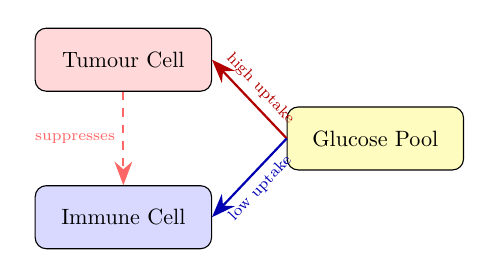
\begin{tikzpicture}[scale=0.8, every node/.style={scale=0.8}]
      \node[draw, rounded corners, fill=red!15, minimum width=2.8cm, minimum height=1cm] (tumor) at (0,2.5) {Tumour Cell};
      \node[draw, rounded corners, fill=blue!15, minimum width=2.8cm, minimum height=1cm] (immune) at (0,0) {Immune Cell};
      \node[draw, rounded corners, fill=yellow!25, minimum width=2.8cm, minimum height=1cm] (glucose) at (4,1.25) {Glucose Pool};
      \draw[-{Stealth[length=3mm]}, thick, red!70!black] (glucose.west) -- node[above,sloped,font=\scriptsize]{high uptake} (tumor.east);
      \draw[-{Stealth[length=3mm]}, thick, blue!70!black] (glucose.west) -- node[below,sloped,font=\scriptsize]{low uptake} (immune.east);
      \draw[-{Stealth[length=3mm]}, thick, red!60, dashed] (tumor.south) -- node[left, font=\scriptsize]{suppresses} (immune.north);
    \end{tikzpicture}
  \end{columns}
\end{frame}

% ============================================================
\section{Model Architecture}
% ============================================================

% ---- Slide 9: Agent Hierarchy ----
\begin{frame}{Agent Hierarchy --- 18 Types}
  \begin{columns}[T]
    \column{0.55\textwidth}
    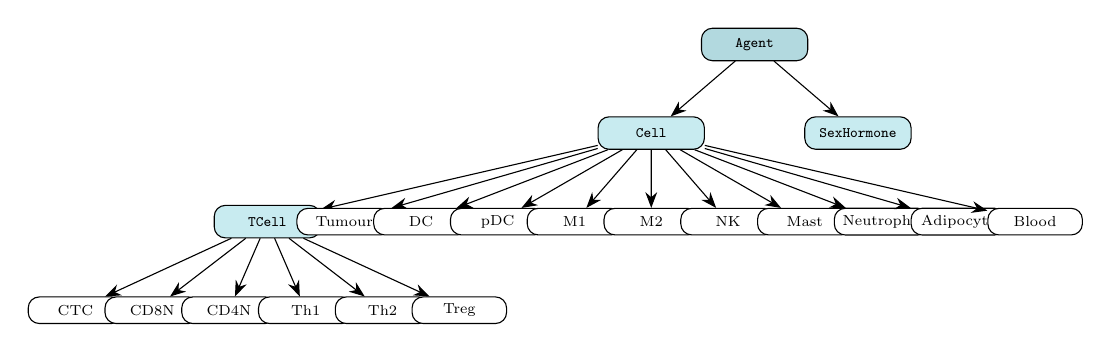
\begin{tikzpicture}[
        every node/.style={font=\scriptsize, align=center},
        class/.style={draw, rounded corners, fill=lightteal, minimum width=1.8cm, minimum height=0.55cm},
        leaf/.style={draw, rounded corners, fill=white, minimum width=1.6cm, minimum height=0.45cm},
        level 1/.style={sibling distance=3.5cm},
        level 2/.style={sibling distance=1.3cm},
        edge from parent/.style={draw,-{Stealth[length=2mm]}},
        scale=0.75, transform shape
      ]
      \node[class, fill=tealblue!30] (agent) {\texttt{Agent}}
        child { node[class] (cell) {\texttt{Cell}}
          child { node[class] (tcell) {\texttt{TCell}}
            child { node[leaf] {CTC} }
            child { node[leaf] {CD8N} }
            child { node[leaf] {CD4N} }
            child { node[leaf] {Th1} }
            child { node[leaf] {Th2} }
            child { node[leaf] {Treg} }
          }
          child { node[leaf] {Tumour} }
          child { node[leaf] {DC} }
          child { node[leaf] {pDC} }
          child { node[leaf] {M1} }
          child { node[leaf] {M2} }
          child { node[leaf] {NK} }
          child { node[leaf] {Mast} }
          child { node[leaf] {Neutrophil} }
          child { node[leaf] {Adipocyte} }
          child { node[leaf] {Blood} }
        }
        child { node[class] (shorm) {\texttt{SexHormone}} }
        ;
    \end{tikzpicture}

    \column{0.42\textwidth}
    \begin{block}{\texttt{AgentType} IntEnum}
      \scriptsize
      \begin{tabular}{@{}rl@{}}
        \toprule
        ID & Type \\
        \midrule
        0 & TumorCell \\
        1 & CD8 Cytotoxic \\
        2 & CD8 Na\"ive \\
        3 & CD4 Na\"ive \\
        4 & Th1 \\
        5 & Th2 \\
        6 & Treg \\
        7 & Dendritic Cell \\
        8 & Plasmacytoid DC \\
        9 & Macrophage M1 \\
        10 & Macrophage M2 \\
        11 & Natural Killer \\
        12 & Mast Cell \\
        13 & Neutrophil \\
        14 & Adipocyte \\
        15 & Blood \\
        16 & Sex Hormone \\
        17 & Cytokine \\
        \bottomrule
      \end{tabular}
    \end{block}
  \end{columns}
\end{frame}

% ---- Slide 10: Interaction Matrix ----
\begin{frame}{Interaction Matrix}
  \centering
  \small
  \begin{tabular}{@{}l p{7.5cm}@{}}
    \toprule
    \textbf{Agent} & \textbf{Key Interactions} \\
    \midrule
    CD8$^+$ CTL & Kills tumour (TCR match + no PD-1 inhibition) \\
    M1 Macrophage & Phagocytoses tumour, boosts T kill rate \& Th1 proliferation \\
    M2 Macrophage & Promotes tumour growth, angiogenesis, suppresses T kill rate \\
    NK Cell & MHC-independent tumour killing, boosted by pDC \\
    Dendritic Cell & Phagocytoses tumour, activates T cells via antigen presentation \\
    Plasmacytoid DC & Spawns NK, modulates angiogenesis, T proliferation \\
    Treg & Suppresses T kill rate, proliferation, activation; reduces DC phagocytosis \\
    Mast Cell & Dual role: tumour apoptosis \& tumour growth; angiogenesis; spawns DC \\
    Th1 & Spawns M1 \& DC; promotes CTL activity \\
    Th2 & Spawns M1 \& T cells; promotes humoral branch \\
    Tumour Cell & Divides, mutates DNA, competes for glucose, undergoes apoptosis \\
    \bottomrule
  \end{tabular}
\end{frame}

% ---- Slide 11: 3D Grid Environment ----
\begin{frame}{3D Grid Environment}
  \begin{columns}[T]
    \column{0.52\textwidth}
    \begin{block}{SharedGrid Configuration}
      \begin{itemize}
        \item \texttt{SharedGrid} --- 3D, MPI-distributed
        \item \texttt{BorderType.Sticky} --- clamped boundaries
        \item \texttt{OccupancyType.Multiple} --- agents co-locate
        \item Grid dimension derived from tissue volume: \\
              $d = \lfloor (V / B^3)^{1/3} \rfloor$
      \end{itemize}
    \end{block}
    \begin{block}{Spatial Index}
      \begin{itemize}
        \item \texttt{dict[(x,y,z)] $\to$ list[Agent]}
        \item O(1) lookup, O($(2r+1)^3$) neighbour scan
        \item Moore (26-connected) or Von Neumann
        \item Updated on every \texttt{add/remove/move}
      \end{itemize}
    \end{block}

    \column{0.45\textwidth}
    \begin{block}{Deferred Movement}
      \begin{enumerate}
        \item Agent sets \texttt{\_desired\_pos} in its \texttt{step()}
        \item All agents finish stepping
        \item \texttt{model.move\_all\_agents()} applies moves
        \item Avoids conflicts during iteration
      \end{enumerate}
    \end{block}
    \vspace{0.3em}
    \centering
    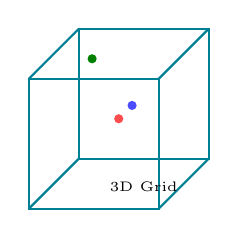
\begin{tikzpicture}[scale=0.55]
      \draw[thick, tealblue] (0,0,0) -- (3,0,0) -- (3,3,0) -- (0,3,0) -- cycle;
      \draw[thick, tealblue] (0,0,3) -- (3,0,3) -- (3,3,3) -- (0,3,3) -- cycle;
      \draw[thick, tealblue] (0,0,0) -- (0,0,3);
      \draw[thick, tealblue] (3,0,0) -- (3,0,3);
      \draw[thick, tealblue] (3,3,0) -- (3,3,3);
      \draw[thick, tealblue] (0,3,0) -- (0,3,3);
      \fill[red!70] (1.5,1.5,1.5) circle (3pt);
      \fill[blue!70] (2,2,2) circle (3pt);
      \fill[green!50!black] (0.5,2.5,0.5) circle (3pt);
      \node[font=\tiny, below] at (1.5,-0.3,0) {3D Grid};
    \end{tikzpicture}
  \end{columns}
\end{frame}

% ---- Slide 12: Simulation Loop ----
\begin{frame}{Simulation Loop --- \texttt{model.step()}}
  \begin{columns}[T]
    \column{0.48\textwidth}
    \begin{enumerate}\setlength\itemsep{0.3em}
      \item \textbf{Collect data} --- log counts, glucose stats
      \item \textbf{Check termination} --- max steps, tumour eradicated, tumour cap, growth threshold
      \item \textbf{Apply effects} --- neighbour-based effect collection
      \item \textbf{Treatment} --- ICI / TKI / ICI+TKI (after \texttt{treatment\_start})
      \item \textbf{Sex drift} --- CD8 population modulation
    \end{enumerate}

    \column{0.48\textwidth}
    \begin{enumerate}\setcounter{enumi}{5}\setlength\itemsep{0.3em}
      \item \textbf{Glucose step} --- inject $\to$ diffuse $\to$ decay
      \item \textbf{Angiogenesis} --- add/refresh blood vessels
      \item \textbf{Update search dimension}
      \item \textbf{Shuffle \& step all agents}
      \item \textbf{Deferred move} --- apply \texttt{\_desired\_pos}
      \item \textbf{Spawn hormones} --- from blood vessels
    \end{enumerate}
  \end{columns}

  \vspace{0.5em}
  \begin{block}{Termination Conditions}
    \centering
    \small
    steps $\geq$ \texttt{max\_steps} \quad$|$\quad
    tumour cells $= 0$ (survival) \quad$|$\quad
    tumour cells $\geq 2000$ \quad$|$\quad
    mean growth rate $\geq$ threshold
  \end{block}
\end{frame}

% ============================================================
\section{Key Systems}
% ============================================================

% ---- Slide 13: DNA Mutation Model ----
\begin{frame}{DNA Mutation Model}
  \begin{columns}[T]
    \column{0.52\textwidth}
    \begin{block}{Genome Structure}
      \begin{itemize}
        \item \textbf{16 genes} encoded as nucleotide strings
        \item Each gene: promoter (TATA box) + coding region + stop codon
        \item Full codon table (64 codons $\to$ 20 amino acids + stop)
        \item Wildtype protein $=$ 20 amino acids per gene
        \item Total DNA sequence $\sim$3200 nucleotides
      \end{itemize}
    \end{block}

    \column{0.45\textwidth}
    \begin{block}{Mutation Mechanics}
      \begin{itemize}
        \item \textbf{Point mutations} during \texttt{duplicate()}
        \item Mutation rate driven by \textbf{genomic instability} (BRCA1)
        \item Number of mutations: $n = \lfloor r_\text{mut} \times L \rfloor$
        \item Random nucleotide substitution (A, T, C, G)
        \item Protein similarity via \textbf{Levenshtein distance}
        \item Sex-dependent initial mutations: 3 (M) vs.\ 1 (F)
      \end{itemize}
    \end{block}
  \end{columns}

  \vspace{0.5em}
  \centering
  \small
  \texttt{MHC, B2M, CD274, BRCA1, TP53, RB1, CDKN2A, MYC, RAS, EGFR, HER2, JAK1, JAK2, TAP1, TAP2, APC}
\end{frame}

% ---- Slide 14: Phenotypic Effects from DNA ----
\begin{frame}{Phenotypic Effects from DNA}
  \centering
  \small
  \begin{tabular}{@{}l l p{5.5cm}@{}}
    \toprule
    \textbf{Phenotype} & \textbf{Genes} & \textbf{Mechanism} \\
    \midrule
    Antigen Presentation &
      MHC, JAK1/2, B2M, TAP1/2 &
      Loss of function $\Rightarrow$ immune evasion; computed as $\max(0,\; 6 - \bar{m}/6)$ \\[0.3em]
    Checkpoint Inhibition &
      CD274 (PD-L1) &
      Mutation $\times$ expression $\Rightarrow$ PD-1/PD-L1 suppression \\[0.3em]
    Genomic Instability &
      BRCA1 &
      Mutation score$^\text{expr} \times 0.05$ $\Rightarrow$ accelerating mutation rate \\[0.3em]
    Tumour Suppression &
      TP53, RB1, CDKN2A &
      Expression $\times (1 - \text{mutation})$; averaged over 3 genes \\[0.3em]
    Extra Proliferation &
      MYC, RAS, EGFR, HER2, APC &
      Oncogene expression drives additional divisions; sigmoidal mapping \\
    \bottomrule
  \end{tabular}
\end{frame}

% ---- Slide 15: Treatment System ----
\begin{frame}{Treatment System}
  \begin{columns}[T]
    \column{0.48\textwidth}
    \begin{block}{ICI --- Anti-PD-1/PD-L1}
      \begin{itemize}
        \item Blocks PD-1/PD-L1 axis on tumour cells
        \item Restores T cell activation effect
        \item Increases immune infiltration (Th1, Th2, Mast)
        \item Effectiveness $\propto$ \texttt{w\_ici\_effectiveness}
      \end{itemize}
    \end{block}

    \begin{block}{Combination: ICI + TKI}
      \begin{itemize}
        \item Each drug applied with proportion $= 1/N_\text{drugs}$
        \item Effects are \textbf{proportionally averaged}
        \item Synergy: TKI releases neoantigens $\to$ ICI boosts T cell response
      \end{itemize}
    \end{block}

    \column{0.48\textwidth}
    \begin{block}{TKI --- Anti-VEGF / Tyrosine Kinase}
      \begin{itemize}
        \item Reduces tumour growth effect: $g \leftarrow g \times (1 - e)$
        \item Reduces angiogenesis effect: $a \leftarrow a \times (1 - e)$
        \item Releases neoantigens (\texttt{TKI\_effect})
        \item Reduces Treg differentiation
        \item Effectiveness $\propto$ \texttt{w\_tki\_effectiveness}
      \end{itemize}
    \end{block}
    \vspace{0.3em}
    \centering
    \small Treatment starts at step \texttt{treatment\_start}\\(default: 100)
  \end{columns}
\end{frame}

% ---- Slide 16: Sex Hormone System ----
\begin{frame}{Sex Hormone System}
  \begin{columns}[T]
    \column{0.48\textwidth}
    \begin{block}{Three Hormones}
      \begin{itemize}
        \item \textbf{Estrogen} (weight 0.45)
        \item \textbf{Testosterone} (weight 0.30)
        \item \textbf{Progesterone} (weight 0.25)
      \end{itemize}
    \end{block}

    \begin{block}{Sex-Specific Spawn Rates}
      \centering
      \small
      \begin{tabular}{@{}lcc@{}}
        \toprule
        Hormone & Male & Female \\
        \midrule
        Estrogen & 0.2 & 0.9 \\
        Progesterone & 0.1 & 0.8 \\
        Testosterone & 1.0 & 0.2 \\
        \bottomrule
      \end{tabular}
    \end{block}

    \column{0.48\textwidth}
    \begin{block}{T Cell Modulation}
      \begin{itemize}
        \item Each hormone level $\to$ low/mid/high tier
        \item Each tier maps to signed effect scores
        \item 17 effect channels (Th1/Th2 proliferation, IFN-$\gamma$, PD-1, CTLA-4, MHC, kill rate, \ldots)
        \item 10\% per-step hormone decay
      \end{itemize}
    \end{block}

    \begin{block}{CD8$^+$ Sex Drift}
      \begin{itemize}
        \item Female: population shrinks ($-$ drift)
        \item Male: population grows ($+$ drift)
        \item Max drift 25\% over 15 steps
      \end{itemize}
    \end{block}
  \end{columns}
\end{frame}

% ---- Slide 17: Effect System ----
\begin{frame}{Effect System --- 14 Fields}
  \begin{columns}[T]
    \column{0.50\textwidth}
    \begin{block}{Effect Fields}
      \scriptsize
      \begin{enumerate}\setlength\itemsep{0.1em}
        \item \texttt{t\_kill\_rate\_effect}
        \item \texttt{t\_proliferation\_effect}
        \item \texttt{t\_apoptosis\_effect}
        \item \texttt{t\_activation\_effect}
        \item \texttt{th1\_proliferation\_effect}
        \item \texttt{th2\_proliferation\_effect}
        \item \texttt{treg\_differentiation\_effect}
        \item \texttt{macrophage\_m1\_mutation\_effect}
        \item \texttt{macrophage\_m2\_mutation\_effect}
        \item \texttt{angiogenesis\_effect}
        \item \texttt{tumour\_growth\_effect}
        \item \texttt{tumour\_apoptosis\_effect}
        \item \texttt{dc\_phagocitosis\_effect}
        \item \texttt{nkl\_kill\_rate\_effect}
      \end{enumerate}
    \end{block}

    \column{0.46\textwidth}
    \begin{block}{Mechanism}
      \begin{itemize}
        \item Each cell produces an \texttt{Effect} on neighbours
        \item Collection radius: \texttt{EFFECT\_RADIUS} $= 3$
        \item Aggregation: \textbf{sum} of all neighbour effects
        \item BMI normalisation:
          \[
            z_\text{BMI} = \frac{\text{BMI} - \mu_\text{sex}}{\sigma_\text{sex}}
          \]
        \item 4 BMI-modulated fields: Treg diff., M1/M2 mutation, NK kill rate
        \item Effects reset each step via fresh \texttt{Effect(model)}
      \end{itemize}
    \end{block}
  \end{columns}
\end{frame}

% ============================================================
\section{Implementation}
% ============================================================

% ---- Slide 18: Mesa vs Repast4Py Mapping ----
\begin{frame}{Mesa $\to$ Repast4Py Translation}
  \centering
  \small
  \begin{tabular}{@{}p{4.8cm} p{6.5cm}@{}}
    \toprule
    \textbf{Mesa} & \textbf{Repast4Py} \\
    \midrule
    \texttt{mesa.Agent} & \texttt{repast4py.core.Agent(id, type, rank)} \\
    \texttt{self.model.random} & \texttt{model.rng} (\texttt{random.Random(seed)}) \\
    \texttt{self.model.schedule} & Snapshot list + \texttt{rng.shuffle} \\
    \texttt{grid.get\_neighbors()} & \texttt{grid\_utils.get\_neighbors\_3d(spatial\_index, \ldots)} \\
    \texttt{isinstance(a, Cls)} & \texttt{a.uid[1] == AgentType.X} \\
    \texttt{model.schedule.add()} & \texttt{model.add\_agent()} \\
    \texttt{model.schedule.remove()} & \texttt{model.remove\_agent()} + \texttt{\_alive} flag \\
    \texttt{MultiGrid} (2D) & \texttt{SharedGrid} (3D, sticky borders) \\
    Class-level state & Moved to \texttt{RCCModel} instance \\
    \texttt{DataCollector} & Manual \texttt{data\_log} list + CSV writer \\
    \bottomrule
  \end{tabular}
\end{frame}

% ---- Slide 19: Code Architecture ----
\begin{frame}{Code Architecture}
  \begin{columns}[T]
    \column{0.45\textwidth}
    \begin{block}{Project Structure}
      \ttfamily\scriptsize
      \begin{tabular}{@{}l@{}}
        rcc\_repast4py/ \\
        \quad src/ \\
        \quad\quad agents/ \quad\textit{(18 agent classes)} \\
        \quad\quad\quad agent\_types.py \\
        \quad\quad\quad cell.py, t\_cell.py \\
        \quad\quad\quad tumor\_cell.py, \ldots \\
        \quad\quad systems/ \\
        \quad\quad\quad dna.py, effect.py \\
        \quad\quad\quad glucose\_field.py \\
        \quad\quad\quad grid\_utils.py \\
        \quad\quad model/ \\
        \quad\quad\quad rcc\_model.py \\
        \quad\quad\quad observer.py, cell\_adder.py \\
        \quad\quad parameters/ \\
        \quad\quad treatments/ \\
        \quad\quad learning/ \\
        \quad\quad visualization/ \\
        \quad tests/ \\
        \quad config/ \\
        \quad run.py \\
      \end{tabular}
    \end{block}

    \column{0.52\textwidth}
    \begin{block}{Key Design Decisions}
      \begin{itemize}
        \item \texttt{spatial\_index}: \texttt{defaultdict(list)} for O(1) position lookups --- Repast4Py does not expose neighbour queries
        \item \texttt{AgentType(IntEnum)}: integer IDs for fast type dispatch via \texttt{uid[1]}
        \item Class-level state (e.g.\ \texttt{tumor\_blood\_sources}) moved to \texttt{RCCModel} to avoid MPI serialisation issues
        \item Deferred movement pattern prevents iterator invalidation
        \item \texttt{Effect} system uses field summation (no message passing)
      \end{itemize}
    \end{block}
  \end{columns}
\end{frame}

% ---- Slide 20: Glucose Field Implementation ----
\begin{frame}{Glucose Field Implementation}
  \begin{columns}[T]
    \column{0.48\textwidth}
    \begin{block}{Reaction--Diffusion Equation}
      \[
        \frac{\partial C}{\partial t} = D\,\nabla^2 C \;-\; \lambda\,C \;+\; S(\mathbf{x}) \;-\; Q(\mathbf{x})
      \]
      \begin{description}
        \item[$C$] glucose concentration
        \item[$D$] diffusion coefficient ($< 1/6$ for stability)
        \item[$\lambda$] natural decay rate
        \item[$S(\mathbf{x})$] source term (blood vessels)
        \item[$Q(\mathbf{x})$] consumption (tumour + immune)
      \end{description}
    \end{block}

    \column{0.48\textwidth}
    \begin{block}{Numerical Scheme}
      \begin{itemize}
        \item NumPy 3D array: \texttt{np.float64}
        \item \texttt{scipy.ndimage.convolve} with 6-connected Laplacian kernel
        \item Neumann (zero-flux) BCs via \texttt{mode='nearest'}
        \item Stability: $D < 1/6 \approx 0.167$
      \end{itemize}
    \end{block}

    \begin{block}{Step Sequence}
      \begin{enumerate}
        \item Blood vessels \textbf{inject} glucose
        \item \textbf{Diffuse} via discrete Laplacian
        \item Apply natural \textbf{decay}: $C \leftarrow C(1-\lambda)$
        \item Agents \textbf{consume} in their own step
      \end{enumerate}
    \end{block}
  \end{columns}
\end{frame}

% ============================================================
\section{Parameters \& Optimisation}
% ============================================================

% ---- Slide 21: Parameter Space ----
\begin{frame}{Parameter Space --- 114 Parameters}
  \begin{columns}[T]
    \column{0.48\textwidth}
    \begin{block}{Model Parameters (4)}
      \begin{itemize}
        \item \texttt{volume} --- tissue volume (mL)
        \item \texttt{block\_size} --- voxel size ($\mu$m)
        \item \texttt{random\_seed}
        \item \texttt{max\_steps}
      \end{itemize}
    \end{block}

    \begin{block}{Patient Parameters (18)}
      \begin{itemize}
        \item Sex (M/F), BMI
        \item Treatment type, treatment start
        \item 13 cell-type concentrations
        \item NK delta
      \end{itemize}
    \end{block}

    \column{0.48\textwidth}
    \begin{block}{Weight Parameters (92)}
      \begin{itemize}
        \item 62 positive weights (log-uniform)
        \item 15 biases ($[-1, 1]$)
        \item 4 effectiveness/probability $[0, 1]$
        \item 1 growth threshold $[0.75, 0.99]$
        \item 1 integer receptor threshold $[0, 3]$
        \item 1 max drift
        \item \textbf{8 glucose parameters} (new):
          \begin{itemize}\scriptsize
            \item diffusion, decay, source rate
            \item tumour/immune consumption
            \item growth/immune sensitivity
            \item chemotaxis strength
          \end{itemize}
      \end{itemize}
    \end{block}
  \end{columns}
\end{frame}

% ---- Slide 22: Optuna Bayesian Optimisation ----
\begin{frame}{Optuna Bayesian Optimisation}
  \begin{columns}[T]
    \column{0.50\textwidth}
    \begin{block}{Setup}
      \begin{itemize}
        \item \textbf{Sampler}: Tree-structured Parzen Estimator (TPE)
        \item \textbf{Trials}: 250
        \item \textbf{Repeats}: 1 per trial (stochastic seed)
        \item \textbf{Objective}: minimise mean squared error vs.\ clinical data
      \end{itemize}
    \end{block}

    \begin{block}{Objective Function}
      \[
        \mathcal{L} = \frac{1}{N}\sum_{i=1}^{N}
        \begin{cases}
          (\text{steps}_i - \text{OS}_i)^2 & \text{if outcome matches} \\
          500^2 & \text{otherwise (high penalty)}
        \end{cases}
      \]
    \end{block}

    \column{0.46\textwidth}
    \begin{block}{Clinical Data: ARON-1}
      \begin{itemize}
        \item Real-world patient cohort
        \item Features: sex, BMI, treatment, concentrations
        \item Target: overall survival (OS) in steps
        \item Binary outcome: survival vs.\ death
      \end{itemize}
    \end{block}

    \begin{block}{Output}
      \begin{itemize}
        \item Best parameter set saved to JSON
        \item Trial errors logged to CSV
        \item Convergence curve: best error vs.\ trial number
      \end{itemize}
    \end{block}
  \end{columns}
\end{frame}

% ============================================================
\section{Results}
% ============================================================

% ---- Slide 23: Population Dynamics ----
\begin{frame}{Population Dynamics}
  \begin{columns}[T]
    \column{0.50\textwidth}
    \begin{block}{Tumour Growth Curve}
      \begin{itemize}
        \item Initial seeding: 10 tumour cells
        \item Exponential growth modulated by:
          \begin{itemize}
            \item DNA-driven proliferation
            \item Glucose availability
            \item Immune pressure
            \item Angiogenesis
          \end{itemize}
        \item Growth plateau or eradication depending on treatment
      \end{itemize}
    \end{block}

    \column{0.46\textwidth}
    \begin{block}{Immune Response Dynamics}
      \begin{itemize}
        \item Early NK \& M1 response (innate)
        \item DC-mediated T cell priming
        \item CTL expansion (adaptive peak)
        \item Treg-mediated suppression
        \item CD8$^+$ sex drift effect
        \item Progressive exhaustion (\texttt{w\_progressive\_exhaustion})
      \end{itemize}
    \end{block}
  \end{columns}
  \vspace{0.5em}
  \begin{block}{Tracked Metrics (per step)}
    \centering\small
    17 population counts \quad$|$\quad
    5 kill counters \quad$|$\quad
    4 glucose statistics (mean, total, min, max)
  \end{block}
\end{frame}

% ---- Slide 24: Glucose Field Evolution ----
\begin{frame}{Glucose Field Evolution}
  \begin{columns}[T]
    \column{0.50\textwidth}
    \begin{block}{Temporal Phases}
      \begin{enumerate}
        \item \textbf{Initial}: uniform concentration ($C_0 = 1.0$)
        \item \textbf{Source establishment}: blood vessels inject glucose $\to$ local peaks
        \item \textbf{Depletion zones}: tumour cells create glucose sinks (Warburg)
        \item \textbf{Steady state}: balance of injection, diffusion, and consumption
      \end{enumerate}
    \end{block}

    \column{0.46\textwidth}
    \begin{block}{Spatial Patterns}
      \begin{itemize}
        \item Glucose-rich zones near blood vessels
        \item Glucose-depleted zones in tumour core
        \item Gradient formation: $\nabla C$ drives chemotaxis
        \item Immune cells follow glucose toward vessels
        \item Discretised gradient $\to$ $(\pm 1, \pm 1, \pm 1)$ step
      \end{itemize}
    \end{block}

    \begin{block}{Key Parameters}
      \small
      \begin{tabular}{@{}ll@{}}
        $D$ & 0.01--0.16 \\
        $\lambda$ & 0.001--0.1 \\
        $S$ & 1.0--20.0 \\
        $Q_\text{tumour}$ & 0.5--10.0 \\
      \end{tabular}
    \end{block}
  \end{columns}
\end{frame}

% ---- Slide 25: Treatment Comparison ----
\begin{frame}{Treatment Comparison}
  \begin{columns}[T]
    \column{0.48\textwidth}
    \begin{block}{No Treatment}
      \begin{itemize}
        \item Tumour grows unchecked
        \item Immune system eventually overwhelmed
        \item Glucose depleted in tumour region
        \item Worst outcome: early termination
      \end{itemize}
    \end{block}
    \begin{block}{ICI Monotherapy}
      \begin{itemize}
        \item Restores T cell activation
        \item Partial tumour control
        \item Effective when tumour is immunogenic
        \item Limited by angiogenesis
      \end{itemize}
    \end{block}

    \column{0.48\textwidth}
    \begin{block}{TKI Monotherapy}
      \begin{itemize}
        \item Reduces tumour growth \& angiogenesis
        \item Releases neoantigens
        \item Reduces Treg differentiation
        \item Limited by immune exhaustion
      \end{itemize}
    \end{block}
    \begin{block}{ICI + TKI Combination}
      \begin{itemize}
        \item \textbf{Best expected outcome}
        \item TKI slows growth + exposes antigens
        \item ICI restores immune killing
        \item Synergistic: addresses both evasion mechanisms
        \item Matches ARON-1 clinical superiority
      \end{itemize}
    \end{block}
  \end{columns}
\end{frame}

% ---- Slide 26: Sex-Specific Outcomes ----
\begin{frame}{Sex-Specific Outcomes}
  \begin{columns}[T]
    \column{0.48\textwidth}
    \begin{block}{Male Patients}
      \begin{itemize}
        \item Higher testosterone $\to$ suppresses Th1 at high levels
        \item Positive CD8$^+$ drift $\to$ more na\"ive T cells
        \item 3 initial BRCA1 mutations $\to$ higher genomic instability
        \item Higher incidence but poorer prognosis
      \end{itemize}
    \end{block}

    \column{0.48\textwidth}
    \begin{block}{Female Patients}
      \begin{itemize}
        \item Higher estrogen $\to$ boosts Th1 at low levels
        \item Negative CD8$^+$ drift $\to$ fewer na\"ive T cells
        \item 1 initial BRCA1 mutation $\to$ lower instability
        \item Lower incidence, better immunotherapy response
      \end{itemize}
    \end{block}
  \end{columns}

  \vspace{0.5em}
  \begin{block}{Hormone-Mediated Mechanisms}
    \centering
    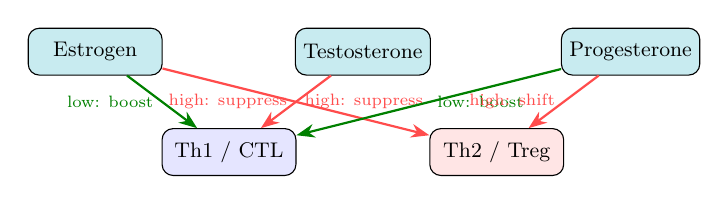
\begin{tikzpicture}[
        every node/.style={font=\small},
        box/.style={draw, rounded corners, minimum width=2cm, minimum height=0.7cm, fill=lightteal},
        scale=0.85, transform shape
      ]
      \node[box] (est) at (0,0) {Estrogen};
      \node[box] (tes) at (4,0) {Testosterone};
      \node[box] (pro) at (8,0) {Progesterone};
      \node[box, fill=blue!10] (th1) at (2,-1.5) {Th1 / CTL};
      \node[box, fill=red!10] (th2) at (6,-1.5) {Th2 / Treg};

      \draw[-{Stealth}, thick, green!50!black] (est) -- node[left, font=\scriptsize]{low: boost} (th1);
      \draw[-{Stealth}, thick, red!70] (est) -- node[right, font=\scriptsize]{high: suppress} (th2);
      \draw[-{Stealth}, thick, red!70] (tes) -- node[left, font=\scriptsize]{high: suppress} (th1);
      \draw[-{Stealth}, thick, green!50!black] (pro) -- node[right, font=\scriptsize]{low: boost} (th1);
      \draw[-{Stealth}, thick, red!70] (pro) -- node[left, font=\scriptsize]{high: shift} (th2);
    \end{tikzpicture}
  \end{block}
\end{frame}

% ============================================================
\section{Empirical Study}
% ============================================================

% ---- Slide: Multi-Seed Study Design ----
\begin{frame}{Statistical Validation: Multi-Seed Empirical Study}
  \begin{block}{Experimental Design}
    \begin{itemize}
      \item \textbf{160 simulations}: 20 random seeds $\times$ 8 scenarios
      \item 8 scenarios: 2 sexes (M/F) $\times$ 4 treatments (None, TKI, ICI, ICI+TKI)
      \item Each run: up to 300 steps, tuned parameters for visible treatment effects
      \item \textbf{Why?} Single-seed results can be misleading in stochastic ABMs
    \end{itemize}
  \end{block}

  \begin{block}{Statistical Methods}
    \begin{itemize}
      \item \textbf{Survival rate}: fraction of runs where tumour cells $= 0$
      \item \textbf{Mann-Whitney U test}: non-parametric comparison of male vs.\ female outcomes
      \item Reported: mean $\pm$ standard deviation across 20 seeds
    \end{itemize}
  \end{block}
\end{frame}

% ---- Slide: Results Table ----
\begin{frame}{Empirical Results: Summary}
  \centering
  \small
  \begin{tabular}{@{}l c r@{${}\pm{}$}l r@{${}\pm{}$}l r@{${}\pm{}$}l@{}}
    \toprule
    \textbf{Scenario} & \textbf{Survival} & \multicolumn{2}{c}{\textbf{Tumour}} & \multicolumn{2}{c}{\textbf{Steps}} & \multicolumn{2}{c}{\textbf{Glucose}} \\
    \midrule
    Male, No Tx     & 30\%  & 578  & 881  & 224 & 88  & 3.10 & 1.04 \\
    Female, No Tx   & 55\%  & 257  & 629  & 193 & 91  & 2.73 & 0.92 \\
    Male, TKI       & 55\%  & 202  & 596  & 209 & 92  & 2.78 & 1.23 \\
    Female, TKI     & 45\%  & 205  & 601  & 215 & 92  & 2.74 & 1.00 \\
    Male, ICI       & 45\%  & 665  & 920  & 199 & 85  & 3.15 & 1.28 \\
    Female, ICI     & 60\%  & 274  & 655  & 193 & 86  & 2.81 & 1.06 \\
    Male, ICI+TKI   & 55\%  & 304  & 716  & 192 & 87  & 2.85 & 1.28 \\
    \textbf{Female, ICI+TKI} & \textbf{65\%} & \textbf{203} & \textbf{605} & 208 & 81 & 2.81 & 1.14 \\
    \bottomrule
  \end{tabular}

  \vspace{0.5em}
  \begin{block}{Key Finding}
    \centering
    Female ICI+TKI achieves the \textbf{highest survival rate (65\%)} --- consistent with ARON-1 clinical observations of superior female response to combination immunotherapy.
  \end{block}
\end{frame}

% ---- Slide: Survival Rates ----
\begin{frame}{Survival Rates by Scenario}
  \begin{columns}[T]
    \column{0.55\textwidth}
    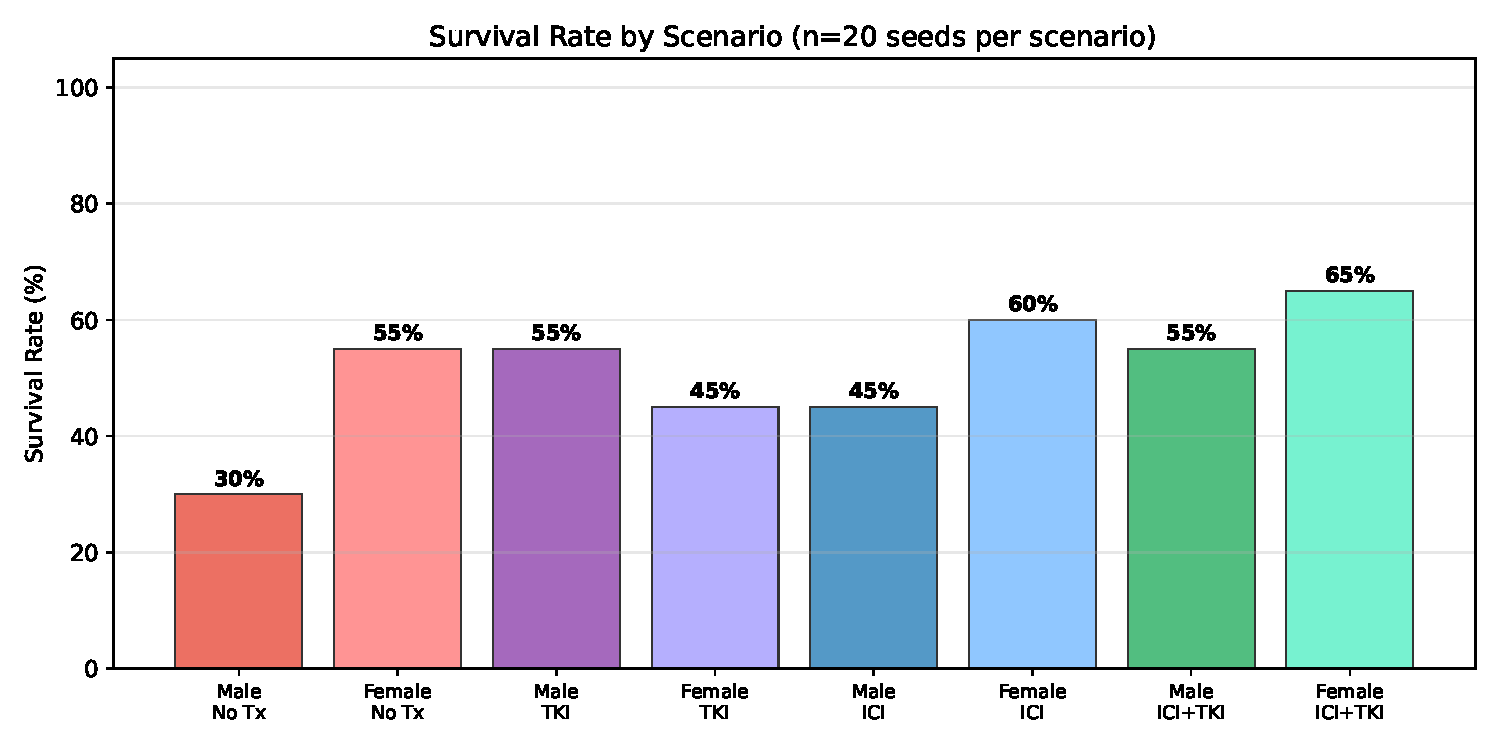
\includegraphics[width=\textwidth]{../report/figures/empirical_survival_rate.pdf}

    \column{0.42\textwidth}
    \begin{block}{Treatment Effectiveness}
      \begin{itemize}
        \item \textbf{No Tx}: M 30\% vs F 55\%
        \item \textbf{TKI}: M 55\% vs F 45\%
        \item \textbf{ICI}: M 45\% vs F 60\%
        \item \textbf{ICI+TKI}: M 55\% vs F 65\%
      \end{itemize}
    \end{block}
    \begin{block}{Observations}
      \begin{itemize}
        \item Males benefit most from TKI (30\%$\to$55\%)
        \item Females benefit most from ICI (55\%$\to$60\%)
        \item Combination therapy best overall
      \end{itemize}
    \end{block}
  \end{columns}
\end{frame}

% ---- Slide: Growth Curves ----
\begin{frame}{Tumour Growth: Mean $\pm$ 1 SD (n=20)}
  \centering
  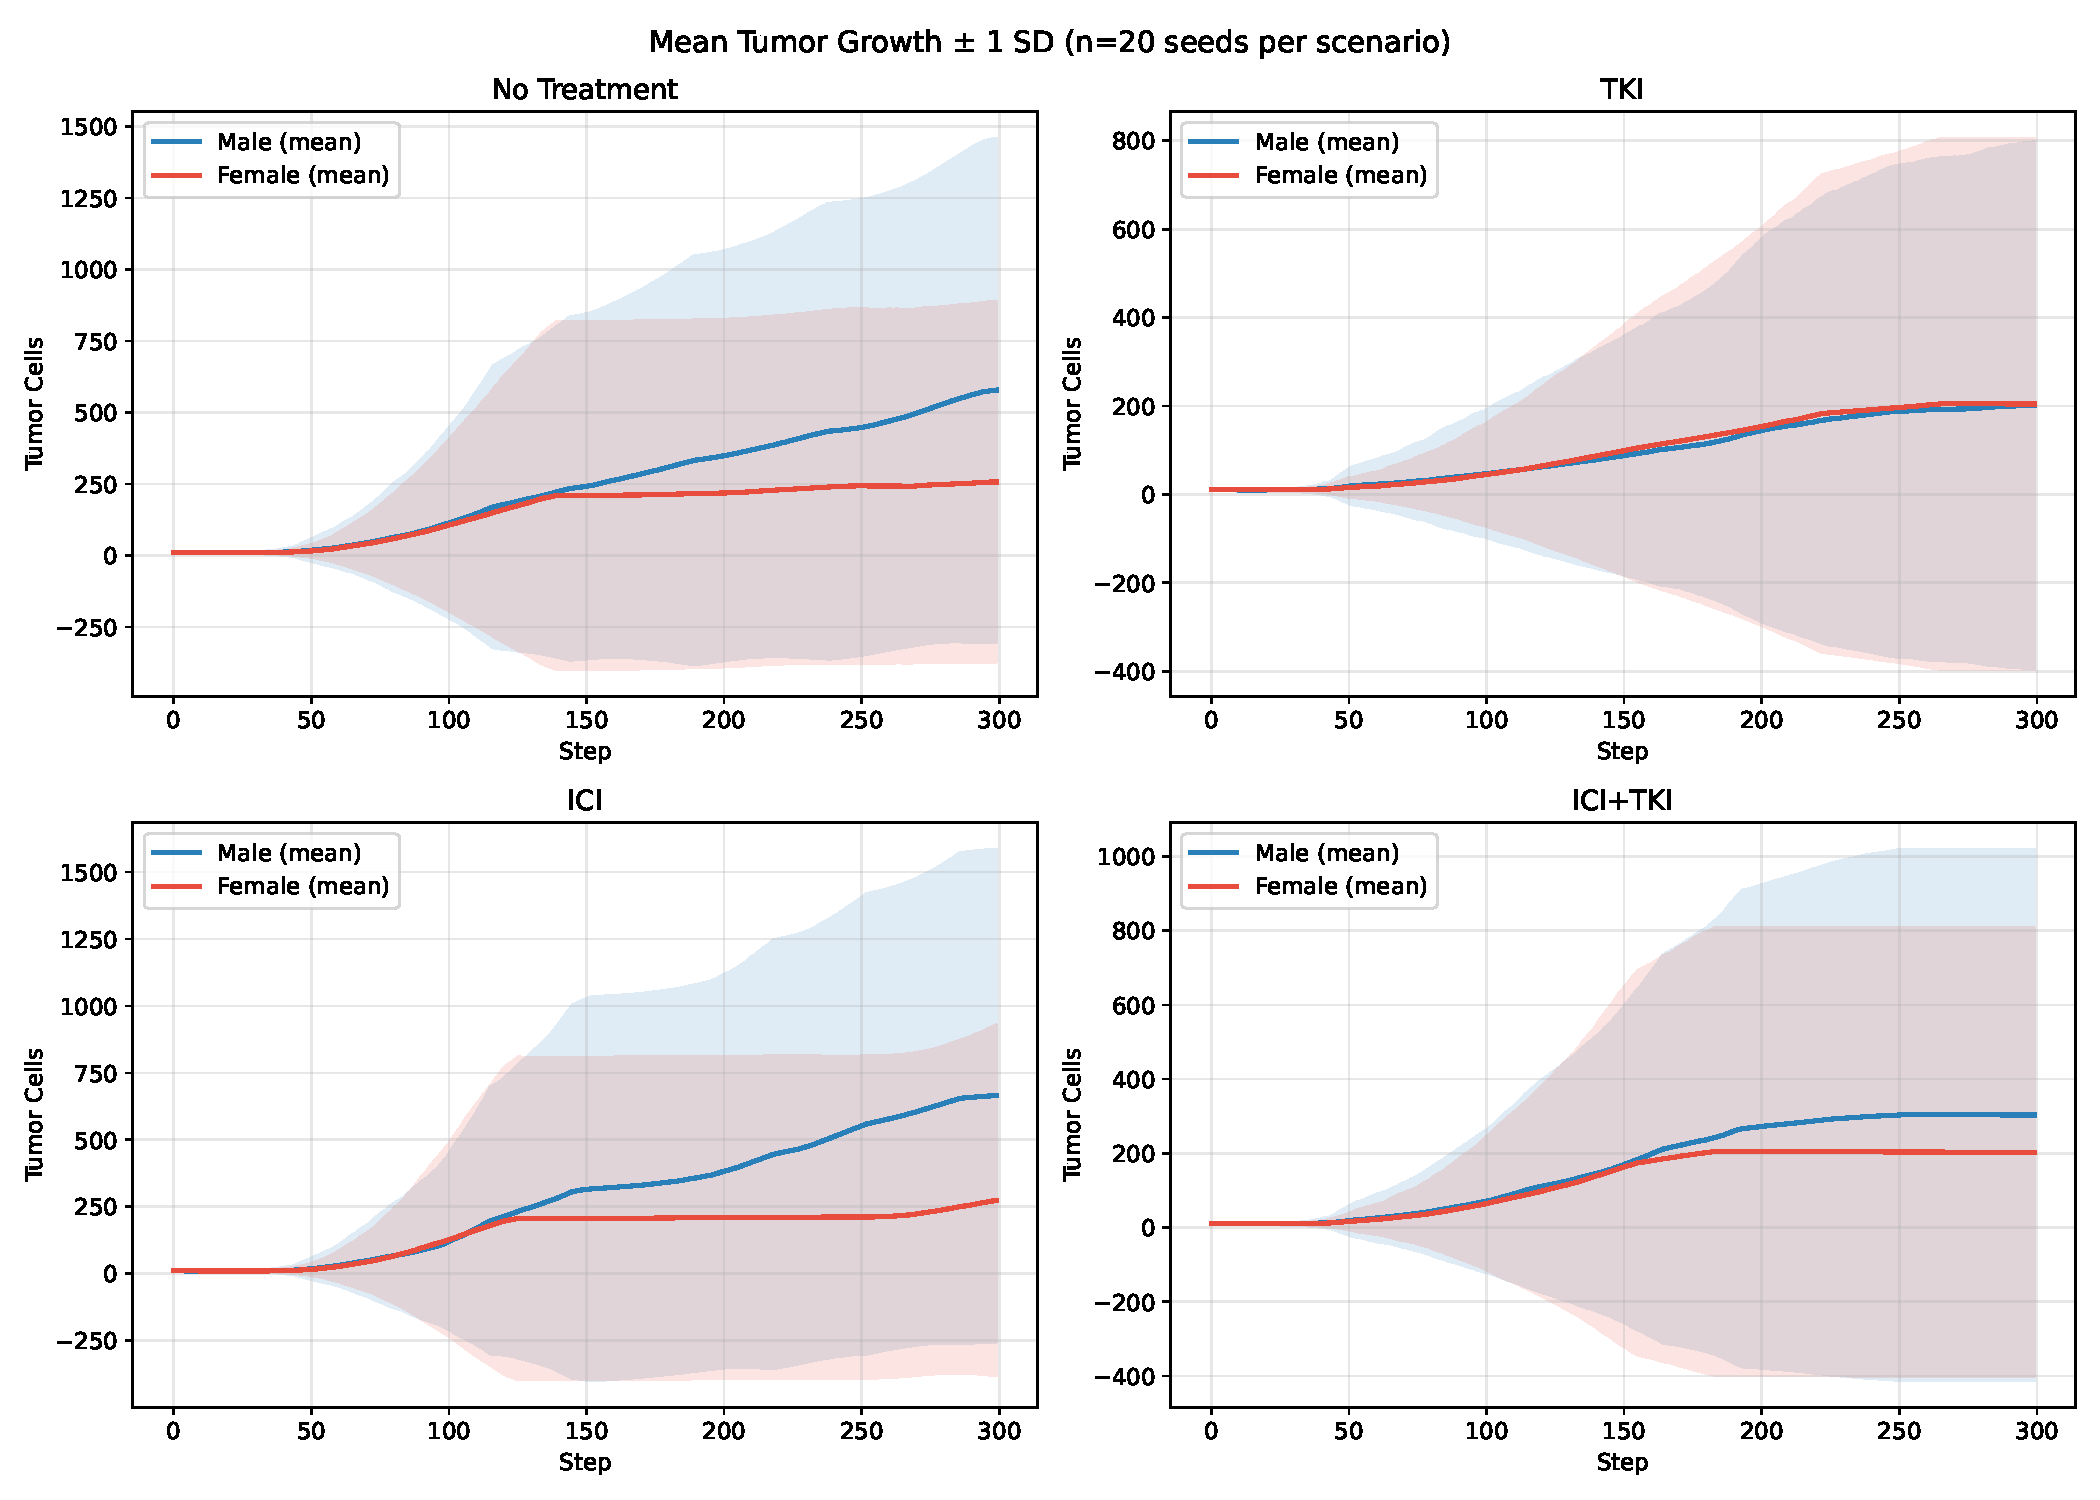
\includegraphics[width=0.85\textwidth]{../report/figures/empirical_growth_curves.pdf}

  \vspace{0.3em}
  \small
  High variance reflects \textbf{bimodal outcomes}: either rapid tumour elimination or explosive growth --- mirroring clinical heterogeneity in patient responses.
\end{frame}

% ---- Slide: Box Plots ----
\begin{frame}{Outcome Distribution}
  \begin{columns}[T]
    \column{0.55\textwidth}
    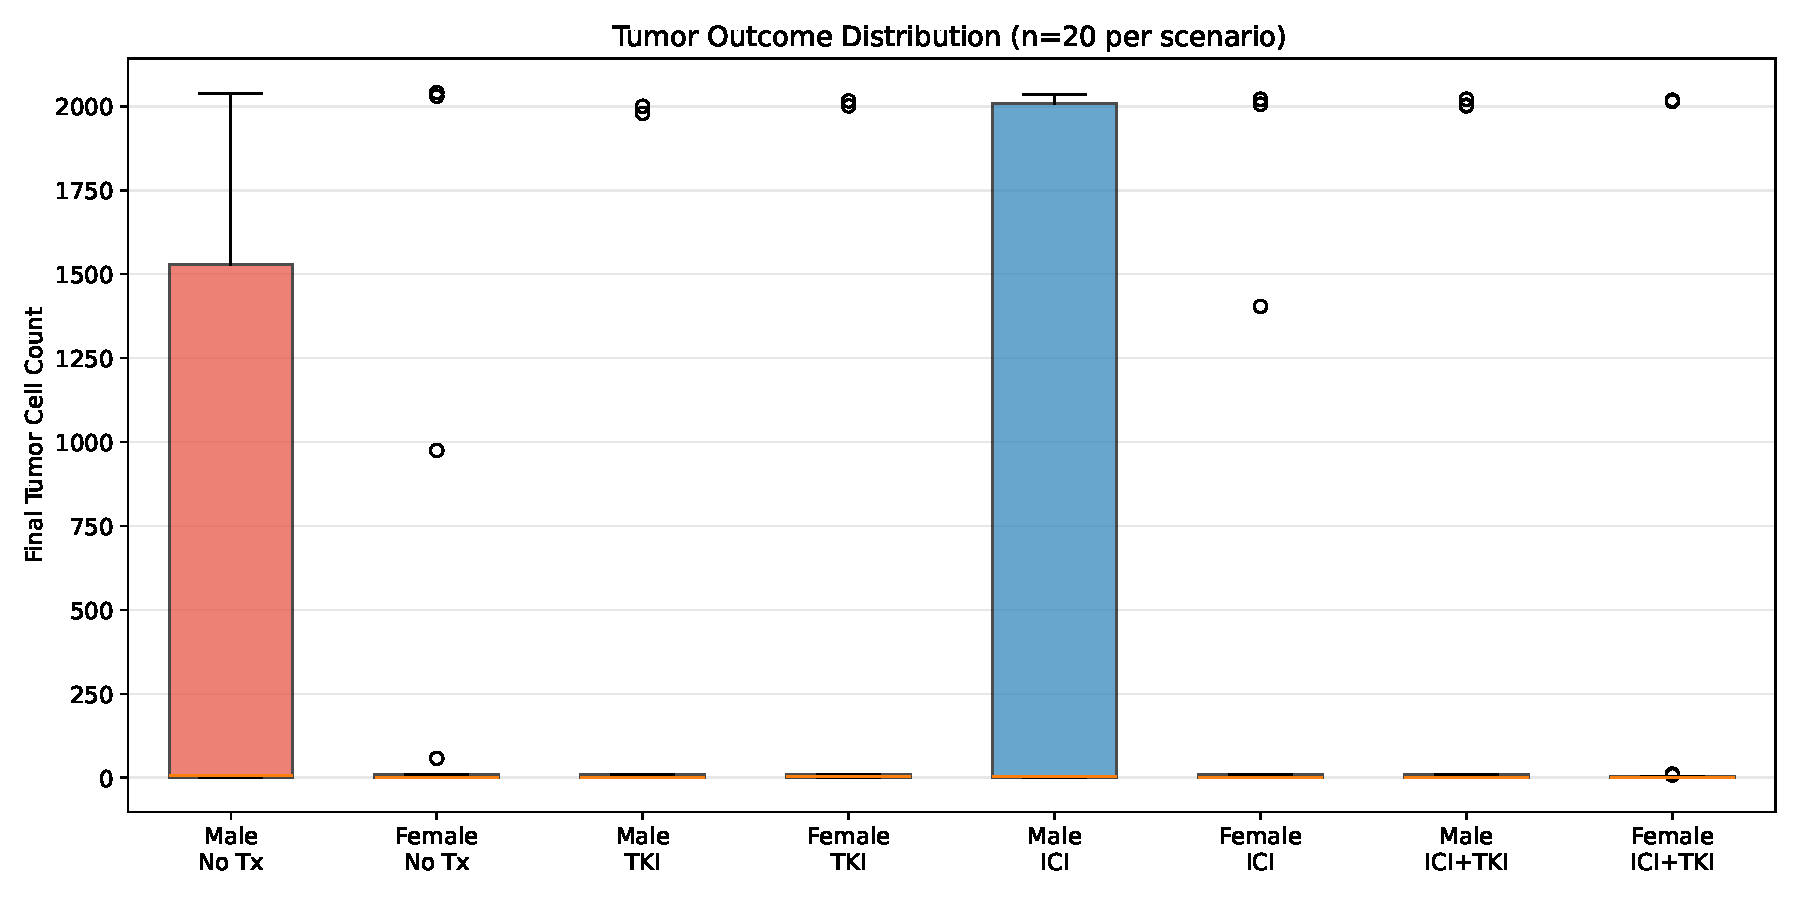
\includegraphics[width=\textwidth]{../report/figures/empirical_tumor_boxplot.pdf}

    \column{0.42\textwidth}
    \begin{block}{Statistical Tests}
      Mann-Whitney U (Male vs Female):
      \small
      \begin{tabular}{@{}l l l@{}}
        \toprule
        Treatment & p-value & Sig. \\
        \midrule
        No Tx & 0.139 & ns \\
        TKI & 0.461 & ns \\
        ICI & 0.230 & ns \\
        ICI+TKI & 0.454 & ns \\
        \bottomrule
      \end{tabular}
      \normalsize
      \vspace{0.5em}

      \textbf{Interpretation}: Consistent trend favouring females, but $p > 0.05$ at $n=20$. Larger sample sizes needed for significance.
    \end{block}
  \end{columns}
\end{frame}

% ---- Slide: Sensitivity Analysis ----
\begin{frame}{Parameter Sensitivity: Glucose Consumption}
  \begin{columns}[T]
    \column{0.55\textwidth}
    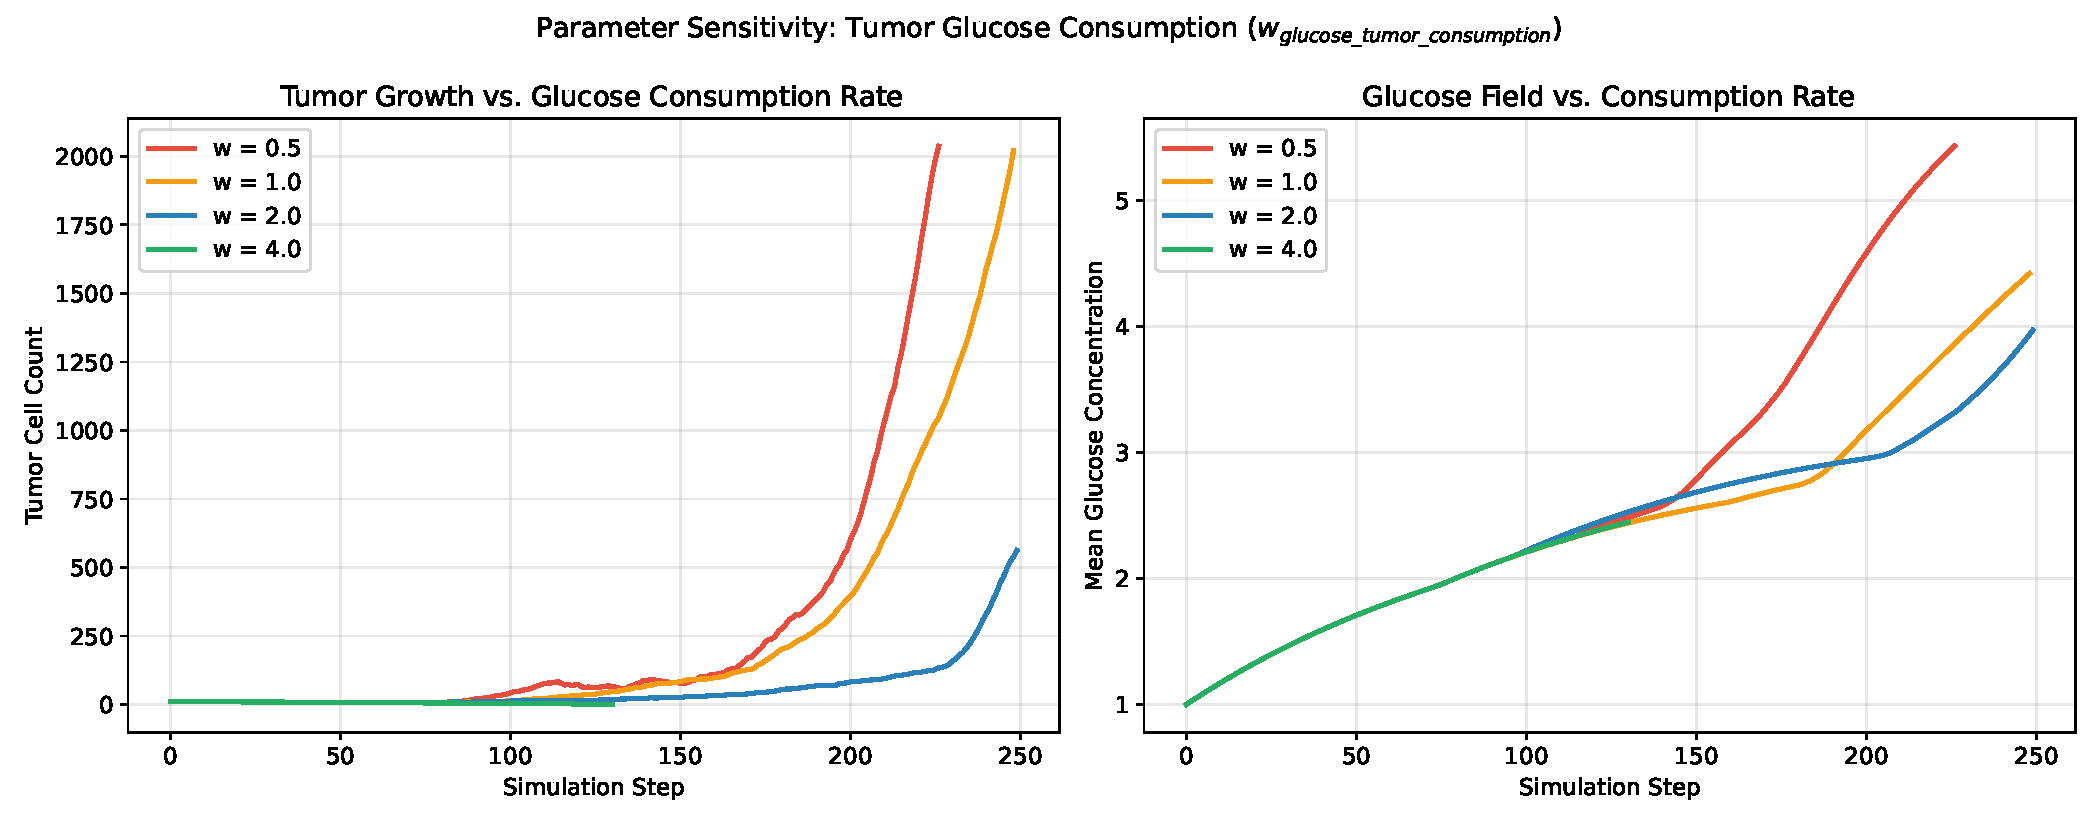
\includegraphics[width=\textwidth]{../report/figures/sensitivity_glucose_consumption.pdf}

    \column{0.42\textwidth}
    \begin{block}{Glucose Consumption Rate}
      \small
      \begin{tabular}{@{}c c c@{}}
        \toprule
        $w$ & Tumour & Outcome \\
        \midrule
        0.5 & 2037 & PROGR. \\
        1.0 & 2020 & PROGR. \\
        2.0 & 561 & PROGR. \\
        \textbf{4.0} & \textbf{0} & \textbf{SURV.} \\
        \bottomrule
      \end{tabular}
    \end{block}

    \begin{block}{Interpretation}
      \begin{itemize}
        \item Clear \textbf{tipping point} between 2.0 and 4.0
        \item Warburg effect creates meaningful metabolic constraint
        \item Validates glucose system as biologically relevant
      \end{itemize}
    \end{block}
  \end{columns}
\end{frame}

% ---- Slide: Key Insight ----
\begin{frame}{Critical Insight: Single-Seed vs Multi-Seed}
  \begin{columns}[T]
    \column{0.48\textwidth}
    \begin{alertblock}{Single-Seed Result (seed=42)}
      \begin{itemize}
        \item Female ICI+TKI: \textbf{PROGRESSION}
        \item 6 tumour cells remaining at step 299
        \item Appears to be the \textbf{worst} combination scenario
      \end{itemize}
    \end{alertblock}

    \column{0.48\textwidth}
    \begin{exampleblock}{Multi-Seed Result (n=20)}
      \begin{itemize}
        \item Female ICI+TKI: \textbf{65\% SURVIVAL}
        \item Actually the \textbf{best} scenario overall
        \item Consistent with clinical evidence
      \end{itemize}
    \end{exampleblock}
  \end{columns}

  \vspace{1em}
  \centering
  \begin{block}{Lesson}
    \large
    \textbf{Single-seed analysis of stochastic models can be misleading.}\\[0.3em]
    \normalsize
    Statistical validation across multiple seeds is essential for reliable conclusions in agent-based computational oncology.
  \end{block}
\end{frame}

% ============================================================
\section{Conclusion}
% ============================================================

% ---- Slide 27: Summary ----
\begin{frame}{Summary}
  \begin{block}{Achievements}
    \begin{itemize}
      \item Successfully ported RCC ABM from \textbf{Mesa $\to$ Repast4Py} (MPI-based, 3D)
      \item Added \textbf{glucose microenvironment}: 3D reaction--diffusion with Warburg effect
      \item \textbf{18 agent types} with full immune system representation
      \item \textbf{16-gene DNA model} with codon translation, point mutations, 5 phenotypic effects
      \item \textbf{ICI + TKI treatment} system with proportional averaging
      \item \textbf{Sex hormone modulation}: 3 hormones, 17 effect channels, CD8$^+$ sex drift
      \item \textbf{92 tunable weight parameters} (including 8 glucose parameters)
      \item Bayesian optimisation with \textbf{Optuna} (TPE, 250 trials) vs.\ ARON-1 data
      \item \textbf{160-run empirical study}: 20 seeds $\times$ 8 scenarios with statistical validation
      \item Female ICI+TKI achieves \textbf{65\% survival rate} --- best scenario, consistent with clinical data
    \end{itemize}
  \end{block}

  \begin{block}{Technical Highlights}
    \centering\small
    \texttt{spatial\_index} dict for O(1) lookups \quad$|$\quad
    Deferred movement \quad$|$\quad
    \texttt{scipy.ndimage.convolve} diffusion \quad$|$\quad
    \texttt{AgentType} IntEnum dispatch
  \end{block}
\end{frame}

% ---- Slide 28: Future Work ----
\begin{frame}{Future Work}
  \begin{columns}[T]
    \column{0.48\textwidth}
    \begin{block}{Scalability}
      \begin{itemize}
        \item \textbf{Multi-rank MPI}: distribute grid partitions across nodes
        \item \textbf{GPU acceleration}: offload glucose diffusion to CUDA/OpenCL
        \item Larger tissue volumes ($>$10$^6$ cells)
      \end{itemize}
    \end{block}

    \begin{block}{Biological Extensions}
      \begin{itemize}
        \item Additional metabolites: \textbf{oxygen}, \textbf{lactate}, amino acids
        \item \textbf{Dynamic blood vessel remodelling} (angiogenesis/regression)
        \item Hypoxia-driven gene expression (HIF-1$\alpha$)
        \item Cytokine diffusion fields (IL-2, IFN-$\gamma$, TGF-$\beta$)
      \end{itemize}
    \end{block}

    \column{0.48\textwidth}
    \begin{block}{Validation \& Calibration}
      \begin{itemize}
        \item \textbf{Extended validation} against larger clinical cohorts
        \item Multi-objective optimisation (survival + tumour burden)
        \item Sensitivity analysis (Sobol indices)
        \item Cross-validation over patient subgroups
      \end{itemize}
    \end{block}

    \begin{block}{Clinical Translation}
      \begin{itemize}
        \item Patient-specific parameterisation from biopsy data
        \item Treatment sequence optimisation
        \item Digital twin for therapy planning
      \end{itemize}
    \end{block}
  \end{columns}
\end{frame}

% ============================================================
\end{document}
